\chapterbegin{Tecnologías y herramientas empleadas}
En este capítulo se detallan las tecnologías que se han empleado para la realización de este proyecto, así como las herramientas software utilizadas, su elección frente a otras alternativas y la labor para la que fueron utilizadas en el ámbito del proyecto.

\section{iOS}
Creado para un hardware en concreto, iOS se ha convertido, en cuanto a software, en la pieza central de Apple desde el año 2007. Actualmente es el núcleo de todos los dispositivos móviles de la compañía: iPhone, iPod Touch y iPad, e incluso de los últimos modelos de Apple TV.

En su lanzamiento, una de las grandes bazas de este Sistema Operativo fue el uso de la tecnología \emph{Multi-Touch}, que permite la manipulación de los objetos en pantalla mediante acciones o \emph{gestos}, tales como \emph{pellizcar}, \emph{tocar} o \emph{deslizar}. Esto produjo un cambio en el paradigma móvil, haciendo que los terminales con teclados físicos hayan ido desapareciendo y, a su vez, el mercado se inunde de \emph{smartphones}, todos ellos con su tienda de aplicaciones.

Las aplicaciones para terceros para iOS aparecieron en marzo de 2008, cuando Apple anunció el lanzamiento del SDK para iOS, así como la \emph{App Store}, la plataforma donde los desarrolladores pueden publicar y comercializar sus aplicaciones diseñadas para iPhone, iPod Touch, iPad, Mac OS X y Apple Watch.

iOS usa una arquitectura en 4 capas, de las cuales las 3 primeras son compartidas con OS X (aunque optimizadas): \emph{Core OS}, \emph{Core Services}, \emph{Media} y \emph{Cocoa Touch}.


\begin{figure}[h]
	\centering
		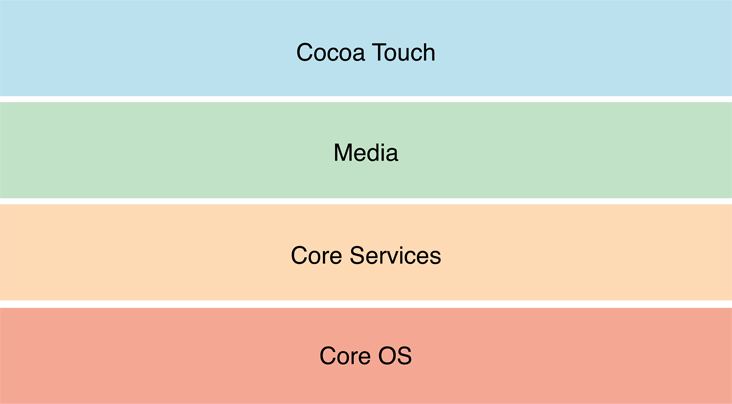
\includegraphics[width=0.5\textwidth]{./img/ios-layers.png}
	\caption{Capas de iOS}
\end{figure}

\subsection*{Core OS}
Contiene los frameworks más básicos para el funcionamiento del Sistema Operativo. Entre ellos podemos encontrar: Core Bluetooth, Network Extension, Security o System.

\subsection*{Core Services}
Contiene los sistemas fundamentales para las aplicaciones. En esta capa podemos acceder a servicios tan imprescindibles en algunas apps como Core Foundation (gestión de hilos, cadenas de caracteres, parseado de documentos XML, manipulación de URLs, etc.), Core Media, Core Location, CFNetwork, Address Book, JavaScript Core, Social, WebKit, etc.

\subsection*{Media}
Contiene todo lo relacionado con audio, vídeo, texto y gráficos. AV Foundation, AV Kit, Core Audio, Core Graphics, Core Text, GLKit, Image I/O o Metal son algunos de los frameworks disponibles en esta capa.

\subsection*{Cocoa Touch}
Siendo la última capa de iOS, su propósito es el de ofrecer todos los recursos para hacer posible la interacción del usuario con las aplicaciones: gráficos, botones y gestos. Algunos de los frameworks en esta última capa son: MapKit, PushKit, Notification Center y UIKit. Éste último puede ser considerado el más importante de esta capa, ya que incorpora todos los elementos básicos de una app, incluyendo su infraestructura, al contener el bucle principal de la aplicación.

\subsection{iPhone OS 1.0, 29 de junio de 2007}
La primera versión de este Sistema Operativo nunca tuvo un nombre definido. Con la salida al mercado del iPhone original, en junio de 2007, el equipo de márketing de Apple únicamente mencionaba que este dispositivo utilizaba una versión simplificada de OS X.

Justo antes de la salida al mercado se anunció que el iPhone únicamente permitiría aplicaciones web desarrolladas por terceras partes, con apenas acceso a diversos sistemas del dispositivo como el hacer una llamada o mandar un correo electrónico \cite{iPhoneWebApps}.

Fue ya en marzo de 2008, con la publicación por parte de Apple del SDK, cuando la compañía empezó a usar el término \emph{iPhone OS} para referirse al Sistema Operativo del iPhone. Gracias a este SDK, terceras partes podrían desarrollar aplicaciones para iPhone y distribuirlas a través de la plataforma exclusiva para este dispositivo: la App Store.

\subsection{iPhone OS 2.0, 11 de julio de 2008}
Con la salida al mercado del iPhone 3G (esta nominación se debe a la posibilidad de poder usar las redes 3G), Apple introdujo una serie de mejoras en la segunda versión del SO, algunas de las cuales centradas en el mundo corporativo, tales como integración con Microsoft Exchange, soporte para lectura de archivos de iWork y Microsoft Office, una gestión mucho más avanzada del correo, notificaciones \emph{push} para las aplicaciones de Apple, etc. También vio un gran avance en temas de seguridad.

En el momento de su presentación, tras apenas 3 meses desde su apertura, el programa de desarrolladores ya había registrado 25.000 solicitudes, aunque al ser un programa en beta cerrada, sólo 4.000 habían sido seleccionados.

\subsection{iPhone OS 3.0, 17 de junio de 2009}
Presentado durante la conferencia mundial de desarrolladores de Apple de 2009 (WWDC) junto al iPhone 3Gs. Más de 1.000 millones de aplicaciones fueron descargadas desde la aparición de la App Store.

Esta versión trajo funciones tan solicitadas como cortar/copiar y pegar, MMS, y muchas mejoras en las APIs notificaciones \emph{push} para aplicaciones de terceros, acceso a la librería de música, 

\subsection{iOS 4, 21 de junio de 2010}

\subsection{iOS 5, 6 de junio de 2011}

\subsection{iOS 6, 11 de junio de 2012}

\subsection{iOS 7, 10 de junio de 2013}

\subsection{iOS 8, 2 de junio de 2014}

\chapterend